\documentclass[a4paper,10pt]{article}
\usepackage{mathtools}
\usepackage{fullpage}
\usepackage{amssymb}
\setcounter{MaxMatrixCols}{20}

\marginparwidth = 10mm

\begin{document}
\title{Oncilla Kinematics}
\author{Pieter-Jan Van de Maele}
\maketitle

\section{Introduction}
Figure \ref{fig:oncilla_geometry} shows a sketch of the geometry of the Oncilla with indication of the used parameters and co\"{o}rdinate systems.
\begin{figure}[h!]
  \centering
  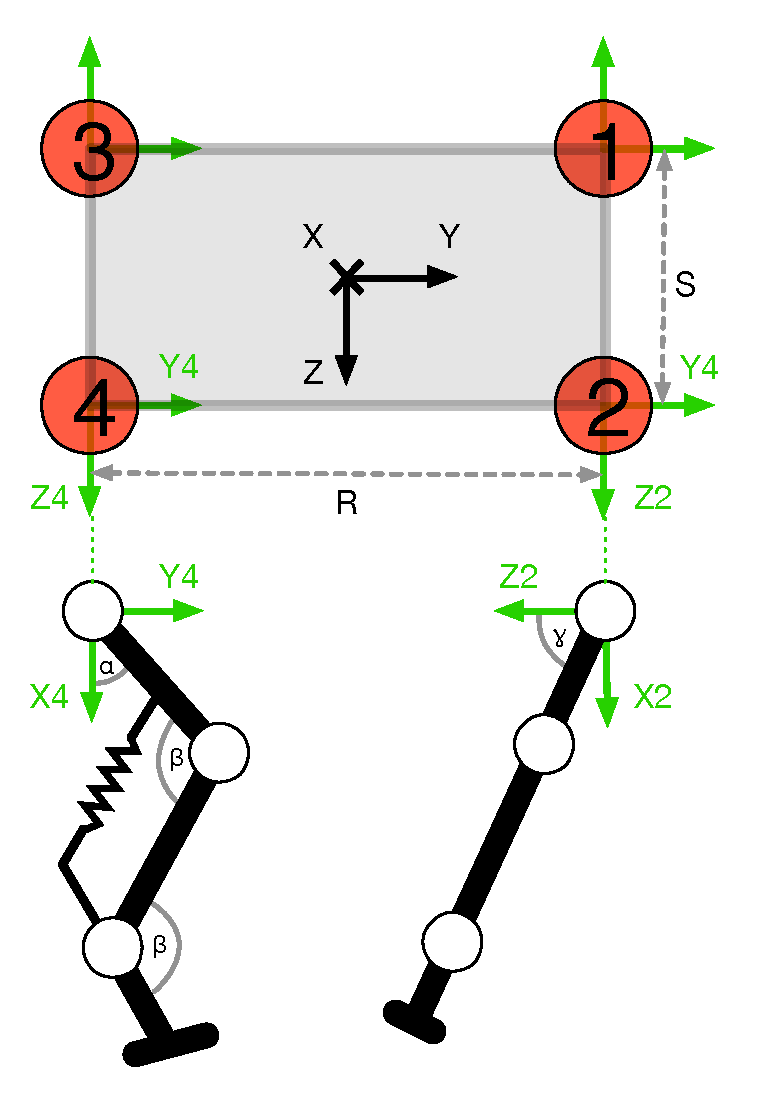
\includegraphics[width=10cm]{Robot}
  \caption{Oncilla geometry}
  \label{fig:oncilla_geometry}
\end{figure}

\section{Forward Kinematics}
Forward kinematics provide the relationship between the values of the actuated joints $\mathbf{q}_{a}$ and the position of the end-effector. $\mathbf{q}_{a} \in \mathbb{R}^{12\times1}$ is given by: \\
\\
$
\mathbf{q}_{a} = \begin{bmatrix}
  \alpha_{1} & \beta_{1} & \gamma_{1} 
  & \alpha_{2} & \beta_{2} & \gamma_{2} 
  & \alpha_{3} & \beta_{3} & \gamma_{3} 
  & \alpha_{4} & \beta_{4} & \gamma_{4} \\
\end{bmatrix}^T
$
\\
\\
For the specification of the forward kinematics, I decided to use the Denavit-Hartenberg convention. The strength of this notation comes from the fact that every link gets its own matrix, which consists of one rotation and one translation. In the end, the mathematical structure remains very readable and similar to the geometric structure. \\
\\
As can be seen in figure \ref{fig:oncilla_geometry}, there are 5 links (3 actuated, 2 unactuated) from the robot center of body (COB) to the end-effector (foot). The 5 matrices are given below.\\
\\
$
\mathbf{DH}_{body} = 
\begin{bmatrix}
       1 & 0 & 0 & Q \\
       0 & 1 & 0 & R \\
       0 & 0 & fl & S \\
       0 & 0 & 0 & 1 
\end{bmatrix}
$
fl = 1 for legs 2, 4 and fl = -1 for legs 1,3
$
\vspace{5mm}
\\
\mathbf{DH}_{servo} = 
\begin{bmatrix}
  \cos{(\gamma-\pi/2)} & 0 & \sin{(\gamma-\pi/2)} & 0 \\
  0 & 1 & 0 & 0 \\
  -\sin{(\gamma-\pi/2)}& 0 & \cos{(\gamma-\pi/2)} & 0 \\
  0 & 0 & 0 & 1 
\end{bmatrix}
\vspace{5mm}
\\
\mathbf{DH}_{hip} = 
\begin{bmatrix}
  \cos\alpha &  -\sin\alpha & 0 & A\cos\alpha \\
  \sin\alpha &  \cos\alpha & 0 & A\sin\alpha \\
  0 & 0 & 1 & 0 \\
  0 & 0 & 0 & 1 
\end{bmatrix}
\vspace{5mm}
\\
\mathbf{DH}_{knee} = 
\begin{bmatrix}
  \cos{(\beta+\pi)} &  -\sin{(\beta+\pi)} & 0 & B\cos{(\beta+\pi)} \\
  \sin{(\beta+\pi)} &  \cos{(\beta+\pi)} & 0 & B\sin{(\beta+\pi)} \\
  0 & 0 & 1 & 0 \\
  0 & 0 & 0 & 1 
\end{bmatrix}
\vspace{5mm}
\\
\mathbf{DH}_{ankle} = 
\begin{bmatrix}
  \cos{(-\beta-\pi)} &  -\sin{(-\beta-\pi)} & 0 & C\cos{(-\beta-\pi)} \\
  \sin{(-\beta-\pi)} &  \cos{(-\beta-\pi)} & 0 & C\sin{(-\beta-\pi)} \\
  0 & 0 & 1 & 0 \\
  0 & 0 & 0 & 1 
\end{bmatrix}
\vspace{5mm}
\\
$
Finally, the forward kinematics can be found by solving following equation: \\
\\
$
\mathbf{F} = \mathbf{DH}_{body}\cdot\mathbf{DH}_{servo}\cdot\mathbf{DH}_{hip}\cdot\mathbf{DH}_{knee}\cdot\mathbf{DH}_{ankle} 
$  
\\
\\
The relative foot positions $\mathbf{P}_{L}$ are thus given by: \\
\\
$
\mathbf{P}_{L_{i}} = 
\begin{bmatrix}
  x_i \\
  y_i \\
  z_i 
\end{bmatrix}
= \mathbf{F}_{1:3} =  
\begin{bmatrix}
  [(A+C)\cos\alpha - B\cos{(\alpha+\beta)}]\sin{\gamma} + Q \\
  (A+C)\sin\alpha - B\sin{(\alpha+\beta)} + R \\
  [(A+C)\cos\alpha - B\cos{(\alpha+\beta)}]\cos{\gamma} + S
\end{bmatrix}
$

\newpage
\section{Single Leg Inverse Kinematics}
The Jacobian for one leg describes the change the foot position makes when a change occurs on the actuators. It is specified as follows:\\
\\
$
\mathbf{J}_{legi} = \dfrac{\partial\mathbf{P}_{L}}{\partial{\mathbf{q}_{a_{j}}}} = \begin{bmatrix}
  \dfrac{\partial{x_i}}{\partial{\alpha_i}} & \dfrac{\partial{x_i}}{\partial{\beta_i}} & \dfrac{\partial{x_i}}{\partial{\gamma_i}} \\[5mm]
  \dfrac{\partial{y_i}}{\partial{\alpha_i}} & \dfrac{\partial{y_i}}{\partial{\beta_i}} & \dfrac{\partial{y_i}}{\partial{\gamma_i}} \\[5mm]
  \dfrac{\partial{z_i}}{\partial{\alpha_i}} & \dfrac{\partial{z_i}}{\partial{\beta_i}} & \dfrac{\partial{z_i}}{\partial{\gamma_i}} \\[5mm]
\end{bmatrix}
\vspace{5mm}
\\
= \begin{bmatrix}
  [-(A+C)\sin\alpha + B\sin{(\alpha+\beta)}]\sin\gamma & B\sin{(\alpha+\beta)}\sin\gamma & [(A+C)\cos\alpha - B\cos{(\alpha+\beta)}]\cos\gamma\\
  (A+C)\cos\alpha - B\cos{(\alpha+\beta)} & -B\cos{(\alpha+\beta)} & 0 \\ 
  [-(A+C)\sin\alpha + B\sin{(\alpha+\beta)}]\cos\gamma & B\sin{(\alpha+\beta)}\cos\gamma & [-(A+C)\cos\alpha + B\cos{(\alpha+\beta)}]\sin\gamma\\
\end{bmatrix} 
$\\
\\\\
When solving the inverse kinematics problem, we have a desired end-effector position, and would like to find the values for the actuators that produce this. With the inverse Jacobian, we can find the following relation: \\
\\
$
\dot{\mathbf{q}}_{legi} = {\mathbf{J}^{-1}_{legi}}\cdot\dot{\mathbf{P}}_{L_{i}} 
$
\\\\
The Oncilla is position controlled. To find the position we run the following algorithm until convergence:
\begin{eqnarray}
&\Delta{\mathbf{x}} := \mathbf{P}_{L_i,current} - \mathbf{P}_{L_i,desired}\\
&\mathbf{q}_{a_j} := \mathbf{q}_{a_j} + \mathbf{J}^{-1}_{legi}\cdot\Delta{\mathbf{x}}\\
&\mathbf{P}_{L_i,current} := ForwardKinematics(\mathbf{q}_{a_j})
\end{eqnarray}

\newpage
\section{Whole Body Inverse Kinematics}
To control the whole robot body, we need to go to a global co\"{o}rdinate system that is no longer attached to the robot. The positions of the robot feet are converted in the global system with the following equation:
\\\\
$
\mathbf{P}_{G} = \mathbf{X}_{B_{n}}+\mathbf{R}_{B}\cdot\mathbf{P}_{L}
$
\\\\
$\mathbf{X}_{B_{n}}$ gives the center of the global coordinate system. $\mathbf{R}_{B}$ specifies the rotation of the co\"{o}rdinate system of the robot relative to the global co\"{o}rdinate system.
\subsection{Rotation Matrix}
The body rotation matrix $\mathbf{R}_{B}$ can be obtained from the kinematic model by making use of the Rodrigues formula. The $x=0$ plane is defined as the plane that goes through three of the robot's feet. So we determine the rotation of the body relative to the ground plane. There is always one foot that does not contribute to the body rotation, this is usually the swing foot. Further logic on the robot will be needed to determine the legs that are responsible for the current rotation.
\vspace{5mm}
\\
$
\mathbf{R}_{B}=\mathbf{I}+\sin{\theta}\mathbf{A}+(1-\cos{\theta})\mathbf{A}^2
$
\vspace{5mm}
\\
$
\theta = \cos^{-1}{\left(\dfrac{(\mathbf{P_{L_1}} - \mathbf{P_{L_2}})\cdot(\mathbf{P_{L_3}}-\mathbf{P_{L_2}})}{\|\mathbf(P_{L_1}-P_{L_2})\|\cdot\|\mathbf(P_{L_3}-P_{L_2})\|}\right)}
$
\vspace{5mm}
\\
$
\mathbf{A} =  \begin{bmatrix}
              0 & -x_3 & x_2 \\ 
              x_3 & 0 & -x_1 \\ 
              -x_2 & x_1 & 0  
              \end{bmatrix}
$
 with 
$
\mathbf{x} = (\mathbf{P_{L_1}} - \mathbf{P_{L_2}})\times(\mathbf{P_{L_3}}-\mathbf{P_{L_2}})
$
\subsection{Center Of Body (COB) Jacobian Control}
To find a control for the COB, I rely on the method discussed in \cite{shkolnik2007inverse}. Here, the assumption is made that the feet on the ground do not move and the robot does not fall over (center of mass, COM, remains inside the support polygon). The COB can then be controlled by simply adjusting the distance of the feet to the center of the body. These distances $L_i$ are given by:   
\\
\\
$L_i = ||\mathbf{P}_{L_i}||$
\\\\
If we then do a little bit of equation-rewriting, we find that:
\\\\
$
\dfrac{\partial{L_i}}{\partial\mathbf{q}_{a}} = \dfrac{\partial{L_i}}{\partial\mathbf{P}_{L_i}}\dfrac{\partial\mathbf{P}_{L_i}}{\partial\mathbf{q}_{a}} = \dfrac{\partial{L_i}}{\partial\mathbf{X}_{B}}\dfrac{\partial\mathbf{X}_B}{\partial\mathbf{q}_a} \implies \mathbf{J}_{X_{B}}=\dfrac{\partial\mathbf{X}_{B}}{\partial\mathbf{q}_{a}} = \left[\dfrac{\partial{L}}{\partial\mathbf{X}_{B}}\right]^+\dfrac{\partial{L}}{\partial\mathbf{P}_{L}}\dfrac{\partial\mathbf{P}_{L}}{\partial\mathbf{q}_{a}}
$
\\
\\\\
With:
\\\\
$
\dfrac{\partial\mathbf{P}_{L}}{\partial\mathbf{q}_{a}} = \begin{bmatrix}
\mathbf{J}_{leg1} & 0 & 0 & 0 \\
0 & \mathbf{J}_{leg2} & 0 & 0 \\
0 & 0 & \mathbf{J}_{leg3} & 0 \\
0 & 0 & 0 & \mathbf{J}_{leg4}  
\end{bmatrix} 
$
\vspace{5mm}
\\
$
\dfrac{\partial{L_{i}}}{\partial{\mathbf{P}_{L}}} = \dfrac{\partial\|\mathbf{P}_{L_{i}}\|}{\partial{\mathbf{P}_{L}}} = \dfrac{[\mathbf{P}_{L_{i}}]^T}{\|\mathbf{P}_{L_{i}}\|}
$
\vspace{5mm}
\\
$
\dfrac{\partial{L_{i}}}{\partial{\mathbf{X}_{B}}} = \dfrac{\partial\|\mathbf{P}_{G_{i}} - \mathbf{X}_{B}\|}{\partial{\mathbf{X}_{B}}} = \dfrac{[\mathbf{X}_{B}-\mathbf{P}_{G_{i}}]^T}{\|\mathbf{X}_{B}-\mathbf{P}_{G_{i}}\|}
$
\vspace{5mm}
\\
\subsection{Jacobian of Body Rotaion}
\subsection{Swing Foot Controller}

\end{document}


